\section{Entropic Relaxation}
\label{sec:entropic}
In their original form, as proposed by Kantorovich~\cite{Kantorovich42}, Optimal Transport distances are not a natural fit for applied problems: they minimize a network flow problem, with a supercubic complexity $(n^3 \log n)$~\citep{Tarjan1997}. Following the work of~\cite{cuturi2013sinkhorn}, we propose an entropic relaxation of $\MOT$, obtain its dual formulation and derive an efficient algorithm to compute an approximation of $\MOT$. 

\subsection{Primal-Dual Formulation}
Let us first extend the notion of Kullback-Leibler divergence for positive Radon measures. Let $\mathcal{Z}$ be a Polish space, for $\mu,\nu\in\mathcal{M}_+(\mathcal{Z})$, we define the generalized Kullback-Leibler divergence as $\KL(\mu||\nu) = \int\log{\frac{d\mu}{d\nu}}d\mu+\int  d\nu - \int d\mu$  if $\mu\ll \nu$, and $+\infty$ otherwise.  We introduce the following regularized version of $\MOT$.

\begin{definition}[Entropic relaxed primal problem]
Let $\mathcal{X}$ and $\mathcal{Y}$ be two Polish spaces, $\mathbf{c}:=(c_i)_{1\leq i\leq N}$ a family of bounded below lower semi-continuous costs lower semi-continuous costs on $\mathcal{X}\times\mathcal{Y}$ and $\bm{\varepsilon}:=(\varepsilon_i)_{1\leq i\leq N}$ be non negative real numbers. For $(\mu,\nu)\in\mathcal{M}_+^{1}(\mathcal{X})\times\mathcal{M}_+^{1}(\mathcal{Y})$, we define the \emph{$\MOT$ regularized primal problem}:
% \begin{align*}
% \MOT_{\mathbf{c}}^{\bm{\varepsilon}}(\mu,\nu):=
% \inf_{\gamma\in \Gamma_{\mu,\nu}^N} \max_{1\leq i\leq N} \left(\int_{\mathcal{X}\times\mathcal{Y}} c_i(x,y)d\gamma_i(x,y)\right)+\sum_{i=1}^N \varepsilon_i\KL(\gamma_i||\mu\otimes \nu)
% \end{align*}
\begin{equation}
\vspace{-0.4cm}
\begin{aligned}
\MOT_{\mathbf{c}}^{\bm{\varepsilon}}(\mu,\nu):= & \inf\limits_{\gamma\in\Gamma_{\mu,\nu}^N}   \max_i\int c_id\gamma_i\label{eq-primal-entrop} 
+\sum_{j=1}^N \varepsilon_j\KL(\gamma_j||\mu\otimes \nu)\notag
\end{aligned}
\end{equation}
% \begin{align}
% \label{eq-primal-entrop}
%  \nonumber \MOT_{\mathbf{c}}^{\bm{\varepsilon}}(\mu,\nu) := & \inf\limits_{(t,\gamma)\in\mathbb{R}\times\Gamma_{\mu,\nu}^N}   t +\sum_{i=1}^N \varepsilon_i\KL(\gamma_i||\mu\otimes \nu) \\
%  &\mathrm{ s.t.}~\forall i, ~ \int_{\mathcal{X}\times\mathcal{Y}}c_id\gamma_i = t
% \end{align}
% As in the standard problem, it is possible to show a property similar to Proposition~\ref{prop:sup-sum-P}:
% \begin{align*}
% \MOT_{\mathbf{c}}^{\bm{\varepsilon}}(\mu,\nu)=
% \sup_{\lambda\in \Delta_N^{+}}\min_{\gamma\in \Gamma_{\mu,\nu}^N}  \sum_{i=1}^N\left(\int_{\mathcal{X}\times\mathcal{Y}} \lambda_ic_i(x,y)d\gamma_i(x,y)+ \varepsilon_i\KL(\gamma_i||\mu\otimes \nu)\right)
% \end{align*}
\end{definition}
Note that here we sum the generalized Kullback-Leibler divergences since our objective is function of $N$ measures in $\mathcal{M}_+(\mathcal{X}\times\mathcal{Y})$. This problem can be compared with the one from standard regularized OT. In the case where $N=1$, we recover the standard regularized OT. For $N\geq 1$, the underlying problem  is $\sum_{i=1}^{N}\varepsilon_i-$strongly convex.
%We also define the dual problem for the entropic regularized problem:
% \begin{definition}[Entropic relaxed dual problem]
% Let $\mathcal{X}$ and $\mathcal{Y}$ be two Polish spaces, $\mathbf{c}:=(c_i)_{1\leq i\leq N}$ a family of nonnegative lower semi-continuous costs on $\mathcal{X}\times\mathcal{Y}$ and $\bm{\varepsilon}:=(\varepsilon_i)_{1\leq i\leq N}$ be non negative real numbers. For $(\mu,\nu)\in\mathcal{M}_1^{+}(\mathcal{X})\times\mathcal{M}_1^{+}(\mathcal{Y})$, we define the entropic regularized dual problem:
% \begin{align*}
% \MOT_{\mathbf{c}}^{\bm{\varepsilon}}(\mu,\nu)= \sup_{\lambda\in\Delta_N^{+}} \sup_{(f,g)\in\mathcal{C}_b(\mathcal{X})\times\mathcal{C}_b(\mathcal{Y})}& \int_{\mathcal{X}} f(x)d\mu(x)+ \int_{\mathcal{Y}} g(y)d\nu(y)\\
% &-\sum_{i=1}^N\varepsilon_i\left( \int_{\mathcal{X}\times\mathcal{Y}} e^{\frac{f(x)+g(y)-\lambda_ic_i(x,y)}{\varepsilon_i}} d\mu(x)d\nu(y)-1\right)
% \end{align*}
% \end{definition}
Moreover, we prove the essential property that as $\bm{\varepsilon}\to 0$, the regularized problem converges to the standard problem. See Appendix~\ref{res:epsto0} for the full statement and the proof. As a consequence, entropic regularization is a consistent approximation of the original problem we introduced in Section~\ref{sec:primal-dual}.
% See Appendix~\ref{prv:epsto0} for the proof.
% \begin{prop}
% \label{prop:epsto0}
% For $(\mu,\nu)\in\mathcal{M}_+^{1}(\mathcal{X})\times\mathcal{M}_+^{1}(\mathcal{Y})$ we have $  \lim\limits_{\bm{\varepsilon}\to0} \MOT_{\mathbf{c}}^{\bm{\varepsilon}}(\mu,\nu) = \MOT_{\mathbf{c}}(\mu,\nu)$.
% % \begin{align*}
% %   \lim_{\bm{\varepsilon}\to0} \MOT_{\mathbf{c}}^{\bm{\varepsilon}}(\mu,\nu) = \MOT_{\mathbf{c}}(\mu,\nu)
% % \end{align*}
% \end{prop}
Next theorem shows that strong duality holds for lower semi-continuous costs and compact spaces. This is the basis of the algorithm we will propose in Section~\ref{sec:algorithms}. See Appendix~\ref{prv:duality-entropic} for the proof.
\begin{thm}[Duality for the regularized problem]
\label{thm:duality-entropic}
Let $\mathcal{X}$ and $\mathcal{Y}$ be two compact Polish spaces, $\mathbf{c}:=(c_i)_{1\leq i\leq N}$ a family of bounded below lower semi-continuous costs on $\mathcal{X}\times\mathcal{Y}$ and $\bm{\varepsilon}:=(\varepsilon_i)_{1\leq i\leq N}$ be non negative numbers. For $(\mu,\nu)\in\mathcal{M}^1_{+}(\mathcal{X})\times\mathcal{M}_+^{1}(\mathcal{Y})$, strong duality holds:
\begin{align}
    \MOT_{\mathbf{c}}^{\bm{\varepsilon}}&(\mu,\nu)=\sup_{\lambda\in\Delta^+_N} \sup\limits_{\substack{f\in\mathcal{C}_b(\mathcal{X})\\g\in\mathcal{C}_b(\mathcal{Y})}} \int fd\mu+ \int gd\nu\label{eq-dual-entrop}\\
 &-\sum_{i=1}^N\varepsilon_i\left( \int e^{\frac{f(x)+g(y)-\lambda_ic_i(x,y)}{\varepsilon_i}} d\mu(x)d\nu(y)-1\right)\notag
\end{align}
and the infimum of the primal problem is attained. 
\end{thm}
% \begin{rmq}\todo{rmplacer cette remarque en disant que min max = min egalitaire pour cout constant! (si cest vrai ofc}
% It is worth noting that the constraint on $\lambda$ to live in $\Delta_N$ in the dual formulation Eq.~\eqref{thm:duality-entropic} of the entropic-based version can be restricted to the simplex $\Delta_N^{+}$. This may have practical interest when deriving an efficient algorithm to compute $\MOT$. See Appendix \ref{res:pgd} for the proof.
% \end{rmq}
As in standard regularized optimal transport there is a link between primal and dual variables at optimum. Let $\gamma^*$ solving the reguralized primal problem and $(f^*,g^*,\lambda^*)$ solving the dual one: $$\forall i,~\gamma_i^* = \exp\left(\frac{f^*+g^*-\lambda^*_i c_i}{\varepsilon_i}\right)\cdot\mu\otimes\nu$$.
\vspace{-0.6cm}
% \subsection{Discrete case}
% We now extend the regularization in the discrete case. 
% Let $a\in\Delta_N^{+}$ and $b\in\Delta_m$ and $\mathbf{C}:=(C_i)_{1\leq i\leq N}\in\left(\mathbb{R}^{n\times m}\right)^N$ be $N$ cost matrices and $\bm{\varepsilon}=(\varepsilon_i)_{1\leq i\leq N}$ be nonnegative real numbers. The discretized regularized primal problem is:
% \begin{align*}
%     \widehat{\MOT}^{\bm{\varepsilon}}_{\mathbf{C}}(a,b)=\inf_{P\in \Gamma_{a,b}^N} \max_{1\leq i\leq N}\langle P_i,C_i\rangle -\sum_{i=1}^N\varepsilon_i \ent(P_i) 
% \end{align*}
% where $\ent(P) = \sum_{i,j}P_{i,j}(\log P_{i,j}-1)$ for $P=(P_{i,j})_{i,j}\in \mathbb{R}_+^{n\times m}$ is the discrete entropy. In the discrete case, strong duality holds thanks to Lagrangian duality and Slater sufficient conditions:
 
% \begin{prop}[Duality for the discrete regularized problem]
% \label{prop:discrete-reg-dual}
% Let $a\in\Delta_N^{+}$ and $b\in\Delta_m$ and $\mathbf{C}:=(C_i)_{1\leq i\leq N}\in\left(\mathbb{R}^{n\times m}\right)^N$ be $N$ cost matrices and $\bm{\varepsilon}:=(\varepsilon_i)_{1\leq i\leq N}$ be non negative reals. Strong duality holds and by denoting $K_i^{\lambda_i} =\exp\left(-\lambda_i C_{i}/\varepsilon_i\right)$, we have
% \begin{align*}
% \widehat{\MOT}_{\mathbf{C}}^{\bm{\varepsilon}}(a,b)=\sup_{\lambda\in\Delta_N^{+}}\sup\limits_{f\in \mathbb{R}^n,~g\in \mathbb{R}^m} \langle f, a\rangle+\langle g,b\rangle-\sum_{i=1}^N\varepsilon_i\langle e^{\mathbf{f}/\varepsilon_i},K_i^{\lambda_i} e^{\mathbf{g}/\varepsilon_i}\rangle.
% \end{align*}
% %In this case optimas are attained for primal and dual problemand: 
% \end{prop}
% The objective function for the dual problem is strictly concave in $(\lambda,f,g)$ but is neither smooth or strongly convex. 

% \todo{Add differentiability w.r.t a and b: enveloppe Moreau theorem}
\subsection{Proposed Algorithms}
\label{sec:algorithms}
% \begin{figure}[t]
% %\vspace{-0.3in}
% \bookboxx{

% \textbf{Input:} $\mathbf{C}=(C_i)_{1\leq i\leq N}$, $a$, $b$, $\varepsilon$, $L$\\
% \textbf{Init:} $f^0\leftarrow \mathbf{1}_n\text{;  }$ $g^0 \leftarrow \mathbf{1}_m\text{;  }$ $\lambda^0 \leftarrow (1/N,...,1/N)\in\mathbb{R}^N$\\
% \textbf{For} $k=1,2,...$ \textbf{do}\\
% \forceindent $K^k \leftarrow \sum_{i=1}^N K_i^{\lambda_i^{k-1}},\quad c_k \leftarrow \langle f^{k-1}, K^k g^{k-1}\rangle,\quad f^{k} \leftarrow \frac{c_k a}{K^{k}g^{k-1}},$

% \forceindent $ d_k \leftarrow\langle f^{k}, K^k g^{k-1}\rangle,\quad g^{k} \leftarrow \frac{d_k b}{ (K^k)^Tf^{k}},\quad \lambda^k \leftarrow \mathrm{Proj}_{\Delta^+_N}\left( \lambda^{k-1} + \frac{1}{L_\lambda}\nabla_{\lambda} F_{\mathbf{C}}^{\varepsilon}(\lambda^{k-1},f^{k},g^{k})\right).$
% }
% \vspace{-0.1in}
% \caption{\small Projected Alternating Minimization Algorithm }
% \label{algo:Proj-Sinkhorn}
% \end{figure}
\begin{algorithm}[ht!]
\SetAlgoLined
\textbf{Input:} $\mathbf{C}=(C_i)_{1\leq i\leq N}$, $a$, $b$, $\varepsilon$, $L_{\lambda}$\\
\textbf{Init:} $f^0\leftarrow \mathbf{1}_n\text{;  }$ $g^0 \leftarrow \mathbf{1}_m\text{;  }$ $\lambda^0 \leftarrow (1/N,...,1/N)\in\mathbb{R}^N$\\
\For{$k=1,2,...$}{$
K^k \leftarrow \sum_{i=1}^N K_i^{\lambda_i^{k-1}},\\
c_k \leftarrow \langle f^{k-1}, K^k g^{k-1}\rangle,~f^{k} \leftarrow \frac{c_k a}{K^{k}g^{k-1}},\\
d_k \leftarrow\langle f^{k}, K^k g^{k-1}\rangle,~g^{k} \leftarrow \frac{d_k b}{ (K^k)^Tf^{k}}, \\
\lambda^k \leftarrow \mathrm{Proj}_{\Delta^+_N}\left( \lambda^{k-1} + \frac{1}{L_\lambda}\nabla_{\lambda} F_{\mathbf{C}}^{\varepsilon}(\lambda^{k-1},f^{k},g^{k})\right).$}
\caption{Projected Alternating Maximization \label{algo:Proj-Sinkhorn}}
\textbf{Result}: $\lambda,f,g$
\end{algorithm}

We can now present algorithms obtained from entropic relaxation to approximately compute the solution of $\MOT$. Let $\mu=\sum_{i=1}^n a_i\delta_{x_i}$ and $\nu=\sum_{j=1}^m b_j\delta_{y_j}$ be discrete probability measures where $a\in\Delta_n^{+}$, $b\in\Delta^+_m$, $\{x_1,...,x_n\}\subset \mathcal{X}$ and $\{y_1,...,y_m\}\subset \mathcal{Y}$. Moreover for all $i\in\{1,\dots,N\}$ and $\lambda>0$, define $\mathbf{C}:=(C_i)_{1\leq i\leq N}\in\left(\mathbb{R}^{n\times m}\right)^N$ with $C_i:=(c_i(x_k,y_l))_{k,l}$ the $N$ cost matrices and $K_i^{\lambda}:=\exp\left(-\lambda C_{i}/\varepsilon\right)$. Assume that  $\varepsilon_1=\dots=\varepsilon_N=\varepsilon$.
%Then the objective~\eqref{eq-primal-entrop} can be written as
% \begin{align*}
%   \widehat{\MOT}^{\bm{\varepsilon}}_{\mathbf{C}}(a,b):=&\inf_{t\in\mathbb{R},P\in \Gamma_{a,b}^N} t -\sum_{i=1}^N\varepsilon_i \ent(P_i)\\
%   &\mathrm{s.t.}~\forall i,
%     ~\langle P_i,C_i\rangle=t
% \end{align*}
% \begin{align*}
%   \widehat{\MOT}^{\bm{\varepsilon}}_{\mathbf{C}}(a,b):=&\inf_{P\in \Gamma_{a,b}^N} \max_i ~\langle P_i,C_i\rangle -\sum_{j=1}^N\varepsilon_j \ent(P_j)
% \end{align*}
% where $\ent(P) = \sum_{i,j}P_{i,j}(\log P_{i,j}-1)$ the discrete Shannon entropy, $\mathbf{C}:=(C_i)_{1\leq i\leq N}\in\left(\mathbb{R}^{n\times m}\right)^N$ are $N$ cost matrices with $C_i:=(c_i(x_k,y_l))_{k,l}$ and the subset of $\left(\mathbb{R}^{n\times m}\right)^N$, representing discrete coupling decomposition:
% \begin{align*}
%   \textstyle \Gamma_{a,b}^N:=\left\{(P_i)_{i=1}^N\text{ s.t. } \sum_i P_i\mathbf{1}_m=a, \sum_i P_i^T\mathbf{1}_n=b \right\}.
% \end{align*}
% Note that, as in standard OT \citep{feydy2018interpolating}, applying the envelope theorem to Eq.\eqref{eq-primal-entrop} gives  the gradients of $ \widehat{\MOT}^{\bm{\varepsilon}}_{\mathbf{C}}(a,b)$ with respect to $a$ and $b$. This property will be useful to compute barycenters in the following.
% \textbf{Differentiability.} As in classical OT \citep{feydy2018interpolating}, applying the envelope theorem to Eq.\eqref{eq-primal-entrop} gives  the gradients of $ \widehat{\MOT}^{\bm{\varepsilon}}_{\mathbf{C}}(a,b)$ with respect to $a$ and $b$. This useful property will be used to compute barycenters in the following.
% In the discrete case, deriving the dual of the problem~\eqref{eq-primal-entrop} leads to the discretized version of Eq.~\eqref{eq-dual-entrop}. 
% In fact deriving the dual of the problem~\eqref{eq-primal-entrop} leads to the discretized version of Eq.~\eqref{eq-dual-entrop}.
Compared to the standard regularized OT,  the main difference here is that the problem contains an additional variable $\lambda\in\Delta_N^{+}$. 
% Note that here we consider the simplex instead of the hyperplane for stability issues. 
When $N=1$, one can use Sinkhorn algorithm. However when $N\geq 2$, we do not have a closed form for updating $\lambda$ when the other variables of the problem are fixed. In order to enjoy from the strong convexity of the primal formulation, we consider instead the dual associated with the equivalent primal problem given when the additional trivial constraint $\mathbf{1}_n^T\left(\sum_i P_i\right)\mathbf{1}_m = 1$  is considered. In that the dual obtained is
\begin{align*}
\label{eq-obj-proj-sin}
    \widehat{\MOT}_{\mathbf{C}}^{\bm{\varepsilon}}(a,b)=&\sup\limits_{\substack{\lambda\in\Delta_N^{+}\\f\in \mathbb{R}^n,~g\in \mathbb{R}^m}} \langle f, a\rangle+\langle g,b\rangle
    -\varepsilon\left[\log\left(\sum_i\langle e^{\mathbf{f}/\varepsilon},K_i^{\lambda_i} e^{\mathbf{g}/\varepsilon}\rangle \right) + 1\right]
\end{align*}
We show that the new objective obtained above is smooth w.r.t $(\lambda,f,g)$. See Appendix~\ref{res:pgd} for the proof. One can  apply the accelerated projected gradient ascent~\citep{beck2009fast,tseng2008accelerated} which enjoys an optimal convergence rate for first order methods of $\mathcal{O}(k^{-2})$ for $k$ iterations.%
\begin{figure*}[ht!]
\vspace{-0.3cm}
\begin{tabular}{ c  c  c  c}
% \vspace{-0.1in}\\
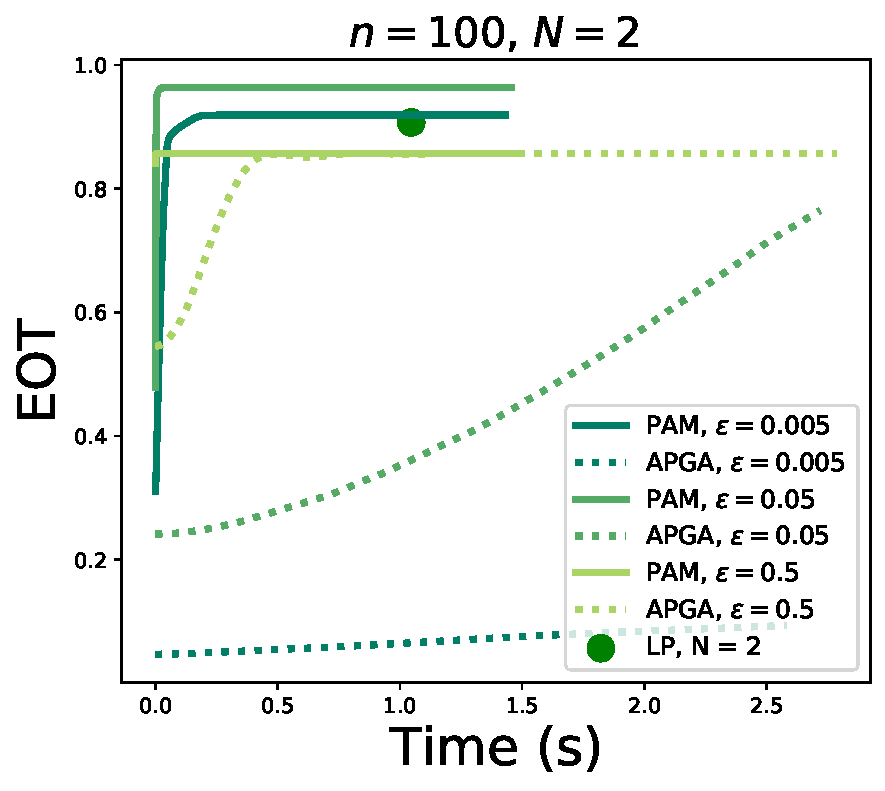
\includegraphics[width=0.28\textwidth%, %height=0.15\textwidth
]{figures/plot_accuracy_vs_time_exp_1.pdf} &
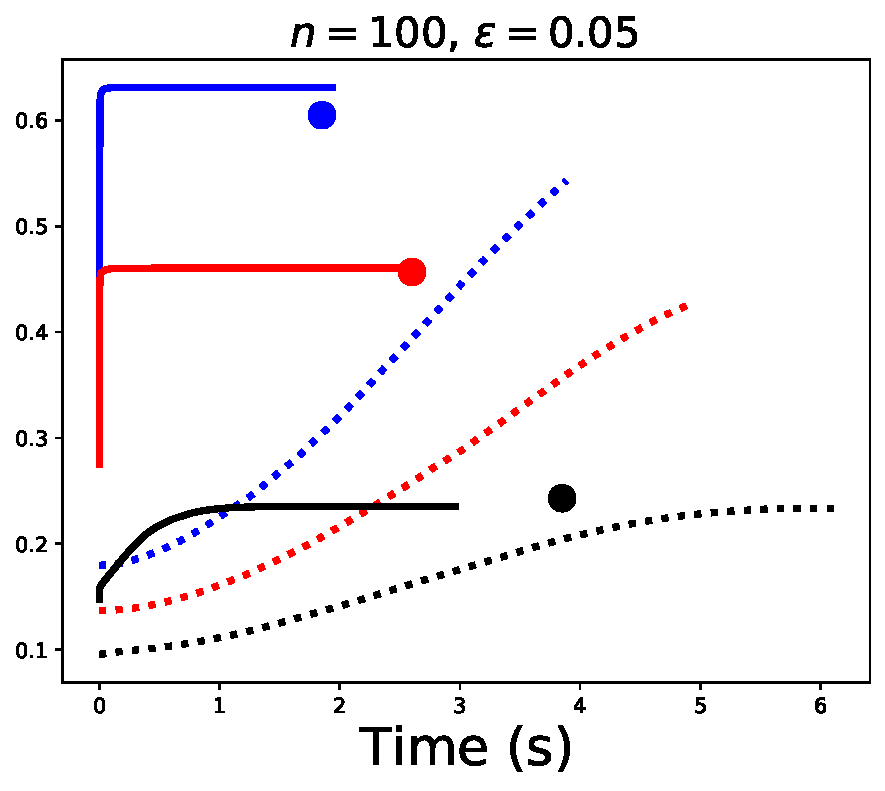
\includegraphics[width=0.28\textwidth%, height=0.15\textwidth
]{figures/plot_accuracy_vs_time_exp_2.pdf}
&
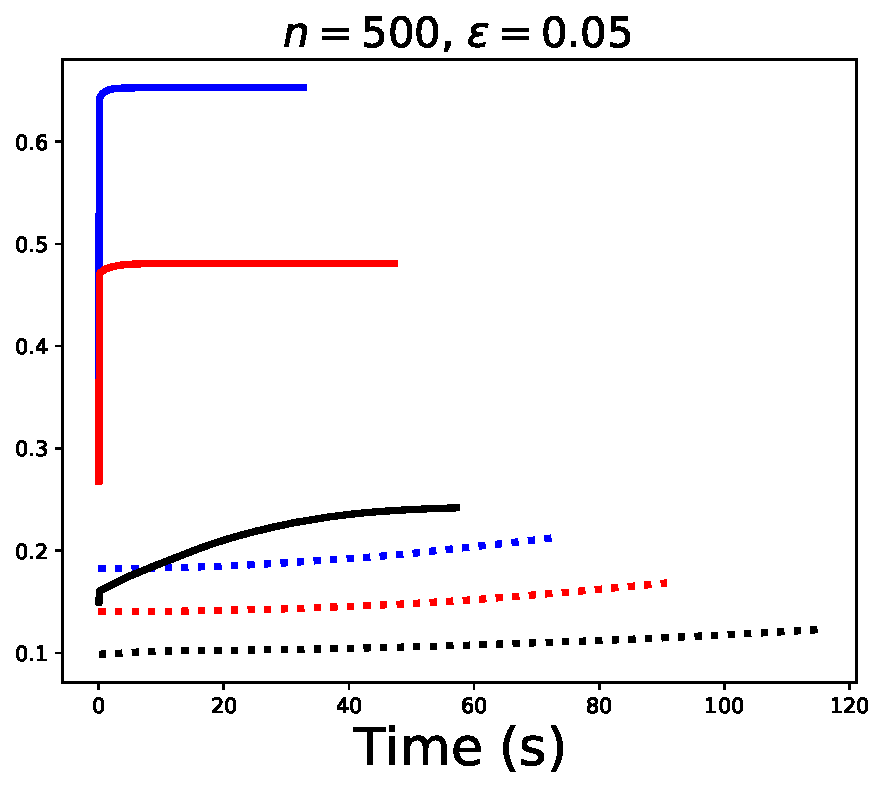
\includegraphics[width=0.28\textwidth%,height=0.15\textwidth
]{figures/plot_accuracy_vs_time_exp_3.pdf} &
\hspace*{-0.6cm}
\raisebox{.9\height}{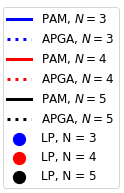
\includegraphics[width=0.08\textwidth%,height=0.15\textwidth
]{figures/legend.png}}
\end{tabular}
\caption{Comparison of the time-accuracy tradeoffs between the different proposed algorithms. \emph{Left:} we consider the case where the number of days is $N=2$, the size of support for both measures is $n=m=100$ and we vary $\varepsilon$ from $0.005$ to $0.5$. \emph{Middle:} we fix $n=m=100$ and the regularization $\varepsilon=0.05$ and we vary the number of days $N$ from 3 to 5. \emph{Right:} the setting considered is the same as in the figure in the middle, however we increase the sample size such that $n=m=500$. Note that in that case, $\textbf{LP}$ is too costly to be computed. \label{fig-seq-OT}}
\end{figure*}

It is also possible to adapt Sinkhorn algorithm to our problem. See Algorithm~\ref{algo:Proj-Sinkhorn}. We denoted by $\mathrm{Proj}_{\Delta_N^+}$ the orthogonal projection on $\Delta_N^+$~\citep{shalev2006efficient}, whose complexity is in $\mathcal{O}(N\log{N})$.  The smoothness constant in $\lambda$ in the algorithm is $L_\lambda = \max_{i}\Vert C_i\Vert_{\infty}^2/\varepsilon$. In practice  Alg.~\ref{algo:Proj-Sinkhorn} gives better results than the accelerated gradient descent. Note that the proposed algorithm differs from the Sinkhorn algorithm in many points and therefore the convergence rates cannot be applied here. Analyzing the rates of a \emph{projected} alternating maximization method is, to the best of our knowledge, an unsolved problem. Further work will be devoted to study the convergence of this algorithm. We illustrate Algorithm~\ref{algo:Proj-Sinkhorn} by showing the convergence of the regularized version of $\MOT$ towards the ground truth when $\varepsilon\to 0$ in the case of the Dudley Metric. See Figure~\ref{fig:result_acc} in Appendix~\ref{appendix-illustrations}.  

% See Appendix~\ref{dis:entropic} for more details on the discrete regularized case and experimental results. 

% In this section, we propose a reformulation of the dual problem to obtain a smooth objective function. We hence develop two algorithms: one based on the same idea that Sinkhorn algorithm (i.e. block coordinate gradient ascent) and one based on an accelerated gradient ascent. Let first prove introduce another discrete duality result:

% \begin{prop}
% \label{prop:algo-dual}
% Let $a\in\Delta_N^{+}$ and $b\in\Delta^+_m$ and $\mathbf{C}:=(C_i)_{1\leq i\leq N}\in\left(\mathbb{R}^{n\times m}\right)^N$ be $N$ cost matrices and $\bm{\varepsilon}:=(\varepsilon,...,\varepsilon)$ where $\varepsilon>0$. Then by denoting $K_i^{\lambda_i} =\exp\left(-\lambda_i C_{i}/\varepsilon\right)$, we have
% \begin{align*}
% \widehat{\MOT}_{\mathbf{C}}^{\bm{\varepsilon}}(a,b)=\sup_{\lambda\in\Delta_N}\sup\limits_{f\in \mathbb{R}^n,~g\in \mathbb{R}^m} F_{\mathbf{C}}^{\varepsilon}(\lambda,f,g):= \langle f, a\rangle+\langle g,b\rangle -\varepsilon\left[\log\left(\sum_{i=1}^N\langle e^{\mathbf{f}/\varepsilon},K_i^{\lambda_i} e^{\mathbf{g}/\varepsilon}\rangle \right) + 1\right].
% \end{align*}
% Moreover, $F_{\mathbf{C}}^{\varepsilon}$ is concave, differentiable and $\nabla F$ is $\frac{\max\left(\max\limits_{1\leq i\leq N}\Vert C_i\Vert_{\infty}^2,2N\right)}{\varepsilon}$ Lipschitz-continuous on $\mathbb{R}^N\times \mathbb{R}^n \times\mathbb{R}^m$.
% \end{prop}
% Denote $L:= \frac{\max\left(\max\limits_{1\leq i\leq N}\Vert C_i\Vert_{\infty}^2,2N\right)}{\varepsilon}$ the  Lipschitz constant of $F_{\mathbf{C}}^{\varepsilon}$. Moreover for all $\lambda\in\mathbb{R}^N$, let $\text{Proj}_{\Delta_N^{+}}(\lambda)$ the unique solution of the following optimization problem $\min_{x\in\Delta_N^{+}} \Vert x - \lambda\Vert_2^2$.
% % \begin{align}
% % \label{prob:proj}
% %     \min_{x\in\Delta_N^{+}} \Vert x - \lambda\Vert_2^2.
% % \end{align}
% Let us now introduce the following algorithm.

% \begin{algorithm}[H]\label{algo:Proj-grad}
% \SetAlgoLined
% \textbf{Input:} $\mathbf{C}=(C_i)_{1\leq i\leq N}$, $a$, $b$, $\varepsilon$, $L$\\
% \textbf{Init:} $f^{-1}=f^0 \leftarrow \mathbf{0}_n\text{;  }$ $g^{-1} = g^0 \leftarrow \mathbf{0}_m\text{;  }$ $\lambda^{-1} = \lambda^0 \leftarrow (1/N,...,1/N)\in\mathbb{R}^N$\\
% \For{$k=1,2,...$}{
% $(v,w,z)^T \leftarrow (\lambda^{k-1},f^{k-1},g^{k-1})^T+\frac{k-2}{k+1}\left((\lambda^{k-1},f^{k-1},g^{k-1})^T- (\lambda^{k-2},f^{k-2},g^{k-2})^T\right);\\
% \lambda^k \leftarrow \text{Proj}_{\Delta_N^+}\left( v + \frac{1}{L}\nabla_{\lambda} F_{\mathbf{C}}^{\varepsilon}(v,w,z)\right);
% \\ (g^k, f^k)^T \leftarrow (w,z)^T + \frac{1}{L}\nabla_{(f,g)} F_{\mathbf{C}}^{\varepsilon}(v,w,z).$}
% \caption{Accelerated Projected Gradient Ascent Algorithm}
% \textbf{Result}: $\lambda,f,g$
% \end{algorithm}

% \cite{beck2009fast,tseng2008accelerated} give us that the acccelerated projected gradient ascent algorithm achieves the optimal rate for first order methods of $\mathcal{O}(1/k^2)$ for smooth functions. To perform the projection we use the algorithm proposed in~\cite{shalev2006efficient} which finds the projection after $\mathcal{O}(N\log(N))$ algebraic operations \citep{wang2013projection}.


% We also propose a projected alternating minimization algorithm as an alternative to the projected gradient which by similar argument can be proved to have sublinear rates. This algorithm is exactly the Sinkhorn algorithm when the number of cost is exaclty $N=1$.

% We cannot directly apply Sinkhorn algorithm since there is a new variable $\lambda$. However we can adapt it by adding a projected gradient step on $\lambda$ in Sinkhorn iterations, which is in short a coordinate gradient ascent for the dual program. For a fixed $\epsilon$, we denote $L$ the smoothness constant of $F_{\mathbf{C}}^{\varepsilon}$ (see details in \todo{add ref}) and  $\mathrm{Proj}_{\Delta_N}$ the orthogonal projection on the affine hyperplane $\Delta_N$ whose complexity is $\mathcal{O}(N)$. We propose Algorithm~\ref{algo:Proj-Sinkhorn} to compute the solution. 



% \begin{algorithm}[H]
% \SetAlgoLined
% \textbf{Input:} $\mathbf{C}=(C_i)_{1\leq i\leq N}$, $a$, $b$, $\varepsilon$, $L$\\
% \textbf{Init:} $f^0\leftarrow \mathbf{1}_n\text{;  }$ $g^0 \leftarrow \mathbf{1}_m\text{;  }$ $\lambda^0 \leftarrow (1/N,...,1/N)\in\mathbb{R}^N$\\
% \For{$k=1,2,...$}{$
% K^k \leftarrow \sum_{i=1}^N K_i^{\lambda_i^{k-1}},\quad c_k \leftarrow \langle f^{k-1}, K^k g^{k-1}\rangle,\quad f^{k} \leftarrow \frac{c_k a}{K^{k}g^{k-1}},
% \\
% d_k \leftarrow\langle f^{k}, K^k g^{k-1}\rangle,\quad g^{k} \leftarrow \frac{d_k b}{ (K^k)^Tf^{k}},\quad \lambda^k \leftarrow \mathrm{Proj}_{\Delta^+_N}\left( \lambda^{k-1} + \frac{1}{L_\lambda}\nabla_{\lambda} F_{\mathbf{C}}^{\varepsilon}(\lambda^{k-1},f^{k},g^{k})\right).$}
% \caption{Projected Alternating Minimization Algorithm \label{algo:Proj-Sinkhorn}}
% \textbf{Result}: $\lambda,f,g$
% \end{algorithm}
% In this section, we propose a reformulation of the dual problem to obtain a smooth objective function. We hence develop two algorithms: one based on the same idea that Sinkhorn algorithm (i.e. block coordinate gradient ascent) and one based on an accelerated gradient ascent. Let first prove introduce another discrete duality result:

% \begin{prop}
% \label{prop:algo-dual}
% Let $a\in\Delta_N^{+}$ and $b\in\Delta^+_m$ and $\mathbf{C}:=(C_i)_{1\leq i\leq N}\in\left(\mathbb{R}^{n\times m}\right)^N$ be $N$ cost matrices and $\bm{\varepsilon}:=(\varepsilon,...,\varepsilon)$ where $\varepsilon>0$. Then by denoting $K_i^{\lambda_i} =\exp\left(-\lambda_i C_{i}/\varepsilon\right)$, we have
% \begin{align*}
% \widehat{\MOT}_{\mathbf{C}}^{\bm{\varepsilon}}(a,b)=\sup_{\lambda\in\Delta_N}\sup\limits_{f\in \mathbb{R}^n,~g\in \mathbb{R}^m} F_{\mathbf{C}}^{\varepsilon}(\lambda,f,g):= \langle f, a\rangle+\langle g,b\rangle -\varepsilon\left[\log\left(\sum_{i=1}^N\langle e^{\mathbf{f}/\varepsilon},K_i^{\lambda_i} e^{\mathbf{g}/\varepsilon}\rangle \right) + 1\right].
% \end{align*}
% Moreover, $F_{\mathbf{C}}^{\varepsilon}$ is concave, differentiable and $\nabla F$ is $\frac{\max\left(\max\limits_{1\leq i\leq N}\Vert C_i\Vert_{\infty}^2,2N\right)}{\varepsilon}$ Lipschitz-continuous on $\mathbb{R}^N\times \mathbb{R}^n \times\mathbb{R}^m$.
% \end{prop}
% Denote $L:= \frac{\max\left(\max\limits_{1\leq i\leq N}\Vert C_i\Vert_{\infty}^2,2N\right)}{\varepsilon}$ the  Lipschitz constant of $F_{\mathbf{C}}^{\varepsilon}$. Moreover for all $\lambda\in\mathbb{R}^N$, let $\text{Proj}_{\Delta_N^{+}}(\lambda)$ the unique solution of the following optimization problem
% \begin{align}
% \label{prob:proj}
%     \min_{x\in\Delta_N^{+}} \Vert x - \lambda\Vert_2^2.
% \end{align}
% Let us now introduce the following algorithm.

% \begin{algorithm}[H]\label{algo:Proj-grad}
% \SetAlgoLined
% \textbf{Input:} $\mathbf{C}=(C_i)_{1\leq i\leq N}$, $a$, $b$, $\varepsilon$, $L$\\
% \textbf{Init:} $f^{-1}=f^0 \leftarrow \mathbf{0}_n\text{;  }$ $g^{-1} = g^0 \leftarrow \mathbf{0}_m\text{;  }$ $\lambda^{-1} = \lambda^0 \leftarrow (1/N,...,1/N)\in\mathbb{R}^N$\\
% \For{$k=1,2,...$}{
% $(v,w,z)^T \leftarrow (\lambda^{k-1},f^{k-1},g^{k-1})^T+\frac{k-2}{k+1}\left((\lambda^{k-1},f^{k-1},g^{k-1})^T- (\lambda^{k-2},f^{k-2},g^{k-2})^T\right);\\
% \lambda^k \leftarrow \text{Proj}_{\Delta_N}\left( v + \frac{1}{L}\nabla_{\lambda} F_{\mathbf{C}}^{\varepsilon}(v,w,z)\right);
% \\ (g^k, f^k)^T \leftarrow (w,z)^T + \frac{1}{L}\nabla_{(f,g)} F_{\mathbf{C}}^{\varepsilon}(v,w,z).$}
% \caption{Accelerated Projected Gradient Ascent Algorithm}
% \textbf{Result}:$\lambda,f,g$
% \end{algorithm}

% \cite{beck2009fast,tseng2008accelerated} give us that the acccelerated projected gradient ascent algorithm achieves the optimal rate for first order methods of $\mathcal{O}(1/k^2)$ for smooth functions. To perform the projection we use the algorithm proposed in~\cite{shalev2006efficient} which finds the solution of (\ref{prob:proj}) after $\mathcal{O}(N\log(N))$ algebraic operations \citep{wang2013projection}.


% We also propose a projected alternating minimization algorithm as an alternative to the projected gradient which by similar argument can be proved to have sublinear rates. This algorithm is exactly the Sinkhorn algorithm when the number of cost is exaclty $N=1$.
% \begin{algorithm}[H]\label{algo:Proj-Sinkhorn}
% \SetAlgoLined
% \textbf{Input:} $\mathbf{C}=(C_i)_{1\leq i\leq N}$, $a$, $b$, $\varepsilon$, $L$\\
% \textbf{Init:} $\alpha^0= \leftarrow \mathbf{1}_n\text{;  }$ $\beta^0 \leftarrow \mathbf{1}_m\text{;  }$ $\lambda^0 \leftarrow (1/N,...,1/N)\in\mathbb{R}^N$\\
% \For{$k=1,2,...$}{$
% K^k \leftarrow \sum_{i=1}^N K_i^{\lambda_i^{k-1}}\\
% c_k \leftarrow \langle \alpha^{k-1}, K^k \beta^{k-1}\rangle\\
% \\
% \alpha^{k} \leftarrow \frac{c_k a}{K^{k-1}\beta^{k-1}}
% \\
% \\
% d_k \leftarrow\langle \alpha^{k}, K^k \beta^{k-1}\rangle
% \\
% \\
% \beta^{k} \leftarrow \frac{d_k b}{ (K^k)^T\alpha^{k}}\\
% \lambda^k \leftarrow \text{Proj}_{\Delta_N}\left( \lambda^{k-1} + \frac{1}{L}\nabla_{\lambda} F_{\mathbf{C}}^{\varepsilon}(\lambda^{k-1},\alpha^{k},\beta^{k})\right).$}
% \caption{Projected Alternating Minimization Algorithm}
% \textbf{Result}:$\lambda,\alpha,\beta$
% \end{algorithm}


% The approximation obtained is [PRIMAL formulation]. Explain that this is always bigger than the true value. 
% \textbf{Illustration.} We evaluate our algorithm on Dudley metric with comparison to the algorithm given by~\cite{sriperumbudur2012empirical}. We show our method is a lot faster and still accurate. We provide a new transport interpretation to this metric of interest. 
% \textbf{Accuracy vs Regularization.} 

% \begin{figure}[h!]
% \centering
% 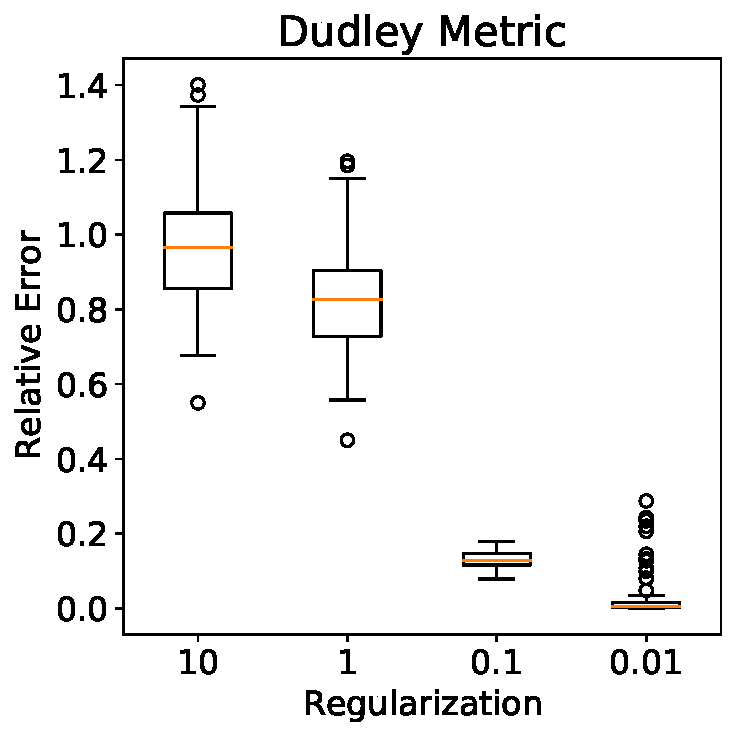
\includegraphics[width=0.8\linewidth]{figures/box_plot_accuracy.pdf}
% \caption{Accuracy vs Regularization.\label{fig:result_acc}}
% \end{figure}
% \begin{figure*}[t]
% \begin{tabular}{@{}c@{}c@{}c@{}c@{}c@{}c@{}c@{}c@{}}
% 
\includegraphics[width=0.14\textwidth]{figures/bary_l2_0.png}&
% 
\includegraphics[width=0.14\textwidth]{figures/bary_wass_1_0.png}&
% 
\includegraphics[width=0.14\textwidth]{figures/bary_wass_1_1.png}&
% 
\includegraphics[width=0.14\textwidth]{figures/bary_wass_1_2.png}&
% 
\includegraphics[width=0.14\textwidth]{figures/bary_wass_1_3.png}&
% 
\includegraphics[width=0.14\textwidth]{figures/bary_wass_1_4.png}&
% 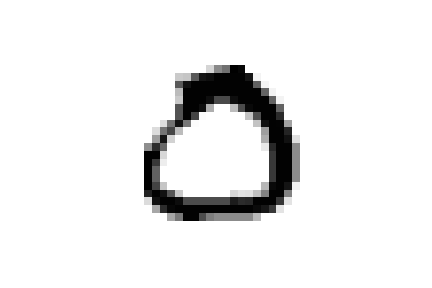
\includegraphics[width=0.14\textwidth]{figures/bary_l2_4.png}
% \\[-.15cm]
% 
\includegraphics[width=0.14\textwidth]{figures/bary_l2_0.png}&
% 
\includegraphics[width=0.14\textwidth]{figures/bary_wass_2_0.png}&
% 
\includegraphics[width=0.14\textwidth]{figures/bary_wass_2_1.png}&
% 
\includegraphics[width=0.14\textwidth]{figures/bary_wass_2_2.png}&
% 
\includegraphics[width=0.14\textwidth]{figures/bary_wass_2_3.png}&
% 
\includegraphics[width=0.14\textwidth]{figures/bary_wass_2_4.png}&
% 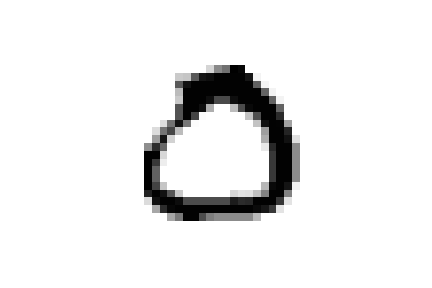
\includegraphics[width=0.14\textwidth]{figures/bary_l2_4.png}
% \\[-.15cm]
% 
\includegraphics[width=0.14\textwidth]{figures/bary_l2_0.png}&
% 
\includegraphics[width=0.14\textwidth]{figures/bary_GOT_0.png}&
% 
\includegraphics[width=0.14\textwidth]{figures/bary_GOT_1.png}&
% 
\includegraphics[width=0.14\textwidth]{figures/bary_GOT_2.png}&
% 
\includegraphics[width=0.14\textwidth]{figures/bary_GOT_3.png}&
% 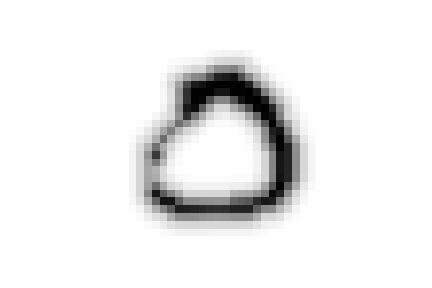
\includegraphics[width=0.14\textwidth]{figures/bary_GOT_4.png}&
% 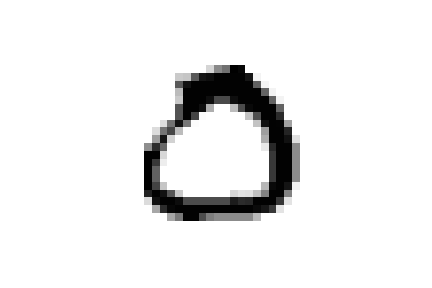
\includegraphics[width=0.14\textwidth]{figures/bary_l2_4.png}
% \end{tabular}
% \caption{It is respectively l2 power 2,l3 power 3 and MOT \label{fig:result_bart_1}}
% \end{figure*}
% \textbf{Illustration with barycenters.} To illustrate $\MOT$, we designed an experiment  with barycenters between two distributions~\citep{agueh2011barycenters}. Although solving costful linear programs to exactly compute such barycenters, we adapt the proposed method from~\cite{CuturiBarycenter} and use Alg.~\ref{algo:Proj-Sinkhorn} to compute them more efficiently. Recall that the algorithm used in~\cite{CuturiBarycenter} is an accelerated  mirror descent which needs the gradient of the $\MOT$ w.r.t. distributions to decrease the overall objective. Figure~\ref{fig:bary-cross} displays the barycenters induced by the $\MOT$ problem compared to standard OT barycenters. We deferred in Appendix~\ref{sec:addexp} additional barycenters experiments on MNIST dataset~\citep{lecunmnist}, and we also provide experiments on the Dudley Metric to show the accuracy of the proposed Alg.~\ref{algo:Proj-Sinkhorn} w.r.t. the regularization $\varepsilon$.

% \begin{figure*}[t]

% \begin{center}

% \begin{tabular}{@{}c@{}c@{}c@{}c@{}c@{}c@{}c@{}c@{}}
% \multirow{3}{*}{
\includegraphics[width=0.10\textwidth]{figures/barycenter_special/croix.png}}&
% 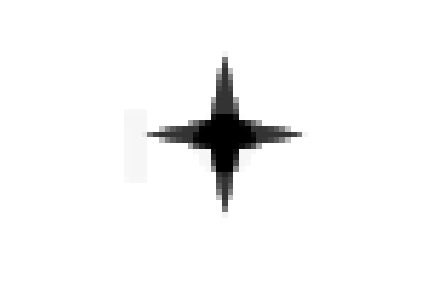
\includegraphics[width=0.12\textwidth]{figures/barycenter_special/bary_wass_1_0.png}&
% 
\includegraphics[width=0.12\textwidth]{figures/barycenter_special/bary_wass_1_1.png}&
% 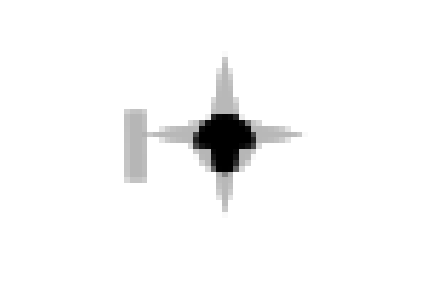
\includegraphics[width=0.12\textwidth]{figures/barycenter_special/bary_wass_1_2.png}&
% 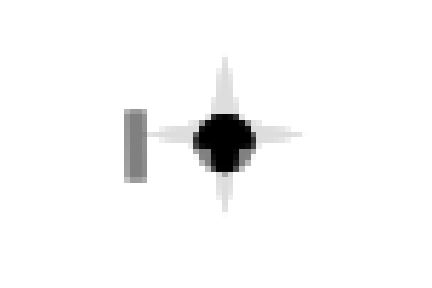
\includegraphics[width=0.12\textwidth]{figures/barycenter_special/bary_wass_1_3.png}&
% 
\includegraphics[width=0.12\textwidth]{figures/barycenter_special/bary_wass_1_4.png}&
% \multirow{3}{*}{
\includegraphics[width=0.10\textwidth]{figures/barycenter_special/dot_trait.png}}
% \\[-.15cm]
% &
% 
\includegraphics[width=0.12\textwidth]{figures/barycenter_special/bary_wass_2_0.png}&
% 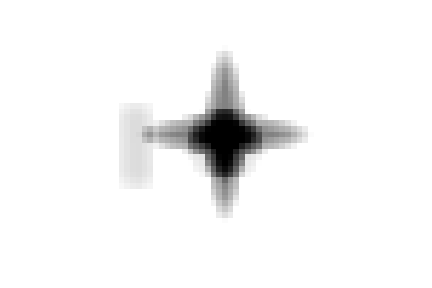
\includegraphics[width=0.12\textwidth]{figures/barycenter_special/bary_wass_2_1.png}&
% 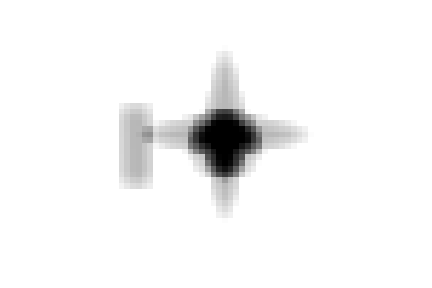
\includegraphics[width=0.12\textwidth]{figures/barycenter_special/bary_wass_2_2.png}&
% 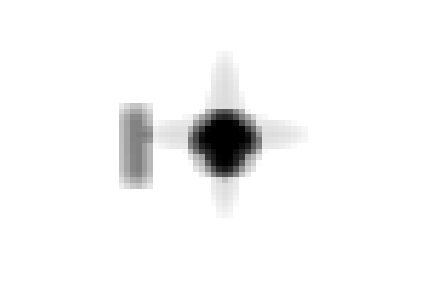
\includegraphics[width=0.12\textwidth]{figures/barycenter_special/bary_wass_2_3.png}&
% 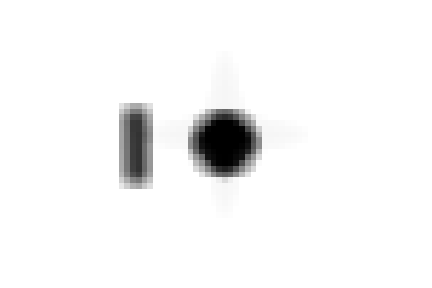
\includegraphics[width=0.12\textwidth]{figures/barycenter_special/bary_wass_2_4.png}&
% %
\includegraphics[width=0.12\textwidth]{figures/barycenter_special/dot_trait.png}
% \\[-.15cm]
% &
% 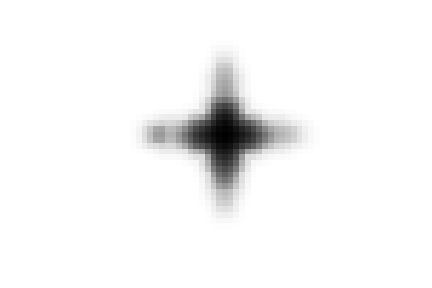
\includegraphics[width=0.12\textwidth]{figures/barycenter_special/bary_GOT_0.png}&
% 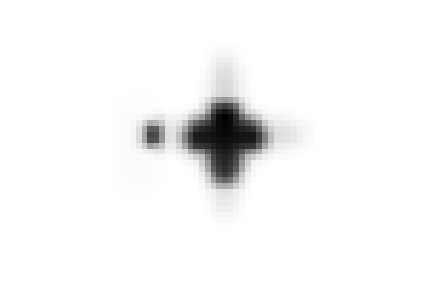
\includegraphics[width=0.12\textwidth]{figures/barycenter_special/bary_GOT_1.png}&
% 
\includegraphics[width=0.12\textwidth]{figures/barycenter_special/bary_GOT_2.png}&
% 
\includegraphics[width=0.12\textwidth]{figures/barycenter_special/bary_GOT_3.png}&
% 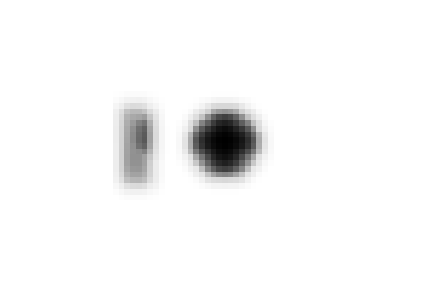
\includegraphics[width=0.12\textwidth]{figures/barycenter_special/bary_GOT_4.png}&
% %
\includegraphics[width=0.12\textwidth]{figures/barycenter_special/dot_trait.png}
% \end{tabular}
% \caption{The two first row starting from the above are Wasserstein barycenters using respectively square $\ell_2$ cost  and the cubic $\ell_3$ taken coordinate by coordinate. The last row represent the $\MOT$ barycenter with respect to these two costs. \textit{From left to right}:  Progressive barycentric transformation of the cross shape to the rectangle and circle shapes. Both shapes are normalized to probability distributions. One can notice that the separation of the cross into the rectangle and the circle induced by the $\MOT$ barycenter is more pronounced than for the ones induced by standard OT barycenters.  \label{fig:bary-cross}}
% \end{center}
% \end{figure*}
% \textbf{Conclusion and future work.} In this paper, we introduced a new variational problem to deal with multiple costs in OT by splitting the transportation problem among the costs such that all costs must contribute equally to the global transport problem. Following the idea of~\cite{cuturi2013sinkhorn}, we derived an entropic relaxation and an efficient algorithm to approximately compute solutions to our problem. 


\section{Other applications of EOT}

\paragraph{Minimal Transportation Time.} Assume there are $N$ internet service providers who propose different debits to transport data across locations, and one needs to transfer data from multiple servers to others, the fastest as possible.   We assume that $c_i(x,y)\geq 0$ corresponds to the transportation time needed by provider $i$ to transport one unit of data from a server $x$ to a server $y$. For instance, the unit of data can be one Megabit. Then $\int c_i d\gamma_i$ corresponds the time taken by provider $i$ to transport $\mu_i=\Pi_{1\sharp}\gamma_i$ to $\nu_i=\Pi_{2\sharp}\gamma_i$. Assuming the transportation can be made in parallel and given a partition of the transportation task $(\gamma_i)_{i=1}^N$, $\max_i\int c_i d\gamma_i$ corresponds to the total time of transport the data $\mu=\Pi_{1\sharp}\sum\gamma_i $ to the locations $\nu=\Pi_{2\sharp}\sum\gamma_i$ according to this partition. Then $\MOT$, which minimizes $\max_i\int c_i d\gamma_i$, is finding the fastest way to transport the data from $\mu$ to $\nu$ by splitting the task among the $N$ internet service providers. Note that at optimality, all the internet service providers finish their transportation task at the same time (see Proposition~\ref{prop:mot-equality}).
 
\paragraph{Sequential Optimal Transport.} Consider the situation where an agent aims to transport goods from some stocks to some stores in the next $N$ days. The cost to transport one unit of good from a stock located at $x$ to a store located at $y$ may vary across the days. For example the cost of transportation may depend on the price of gas, or the daily weather conditions. Assuming that he or she has a good knowledge of the daily costs of the $N$ coming days, he or she may want a transportation strategy such that his or her daily cost is as low as possible. By denoting $c_i$ the cost of transportation the $i$-th day, and given a strategy $(\gamma_i)_{i}^N$, the maximum daily cost is then $\max_i\int c_i d\gamma_i$, and $\MOT$ therefore finds the cheapest strategy to spread the transport task in the next $N$ days such that the maximum daily cost is minimized. Note that at optimality he or she has to spend the exact same amount everyday.


In Figure~\ref{fig-seq-OT} we aim to simulate the Sequential OT problem and compare the time-accuracy trade-offs of the proposed algorithms. Let us consider a situation where one wants to transport merchandises from $\mu = \frac{1}{n}\sum_{i=1}^n  \delta_{x_i}$ to $\nu =\frac{1}{m} \sum_{j=1}^m \delta_{y_j}$ in $N$ days. Here we model the locations  $\{x_i\}$ and $\{y_j\}$ by drawing them independently from two Gaussian distributions in $\mathbb{R}^2$: $\forall i,~x_i\sim \mathcal{N}\left(\begin{psmallmatrix}
3\\
3\\
\end{psmallmatrix},\begin{psmallmatrix}
0 & 1\\
1 & 0 \\
\end{psmallmatrix}\right)$ and $\forall j,~y_j\sim \mathcal{N}\left(\begin{psmallmatrix}
4\\
4\\
\end{psmallmatrix},\begin{psmallmatrix}
1 & -.2\\
-.2 & 1\\
\end{psmallmatrix}\right).$
% \begin{align*}
% \forall~i,j,~x_i\sim \mathcal{N}\left(\begin{psmallmatrix}
% 3\\
% 3\\
% \end{psmallmatrix},\begin{psmallmatrix}
% 0 & 1\\
% 1 & 0 \\
% \end{psmallmatrix}\right),
% ~y_j\sim \mathcal{N}\left(\begin{psmallmatrix}
% 4\\
% 4\\
% \end{psmallmatrix},\begin{psmallmatrix}
% 1 & -.2\\
% -.2 & 1\\
% \end{psmallmatrix}\right).
% \end{align*}
We assume that everyday there is wind modeled by a vector $w\sim \mathcal{U}(B(0,1))$ where $B(0,1)$ is the unit ball in $\mathbb {R}^2$ that is perfectly known in advance. We define the cost of transportation on day $i$ as $c_i(x,y) = \lVert y-x\rVert -0.7 \langle w_i,y-x\rangle$ to model the effect of the wind on the transportation cost. In the following figures we plot the estimates of EOT obtained from the proposed algorithms in function of the runtime for various sample sizes $n$, number of days $N$ and regularizations $\varepsilon$. \textbf{PAM} denotes Alg.~\ref{algo:Proj-Sinkhorn}, \textbf{APGA} denotes Alg.~\ref{algo:Proj-grad} (See Appendix C.4), \textbf{LP} denotes the linear program which solves exactly the primal formulation of the EOT problem. Note that when $\textbf{LP}$ is computable (i.e. $n\leq 100$), it is therefore the ground truth. We show that in all the settings, \textbf{PAM} performs better than $\textbf{APGA}$ and provides very high accuracy with order of magnitude faster than $\text{LP}$. 

